\chapter{Część praktyczna}
\label{chapter:application}

\newglossaryentry{horizon}{name={Horizon},description={Aplikacje internetowa, do zarządzania chmurzę obliczeniową OpenStack}}

Cześć praktyczna pracy dyplomowej dotyczy implementacji oprogramowania typu \textbf{LaaS} (\ref{chapter:monitoring_architecture:laas}).
W założeniu ma ono stanowić część całego stosu oferowanego przez firmę Fujitsu dla kompleksowego monitorowania chmur obliczeniowych.
Niemniej, możliwe jest również wykorzystania części lub całości, do monitoringu standardowych systemów informatycznych. 
Specyficzną oraz wyjątkową cechą części praktycznej, oprócz realizowania jej również na płaszczyźnie zawodowej, jest jej otwartość.
Całość implementacji dostępna jest jako oprogramowania otwarte na licencji \textbf{Apache License V2.0}. Dzięki temu też, autor poniższej pracy dyplomowej, ma możliwość tworzenia aplikacji we współpracy z takimi firmami:
\begin{itemize}
    \item Hewlett Packard,
    \item Time Warner Cable.
\end{itemize}

Implementacja stanowi rozszerzenie projektu monasca, oryginalnie przygotowanego i opublikowanego przez firmę HP.
Całość infrastruktury składa się z następujących programów:
\begin{itemize}
    \item[monasca-api] - REST'owe API, z którym komunikują się pozostałe komponenty, celem zapisywania metryk, alarmów (oraz ich definicji).
    Pozwala także na dostęp do wspomnianych danych.
    \item[monasca-agent] - rozbudowane narzędzie do monitorowania systemu lub aplikacji na maszynie na której został zainstalowany.
    \item[monasca-persister] - prowadzi aktywny nasłuch na kolejce. Wszelkie zmiany stanu na alarmach oraz przekazane metryki, zapisuje,
    poprzez \textbf{monasca-api} do bazy danych.
    \item[monasca-thresh] - jest w stanie, na podstawie zebranych metryk, określić stan w jakim powinien znaleźć się alarm.
    \item[monasca-notification] - na podstawie alarmów, generuje powiadomienie na skonfigurowanego punkty docelowe,
    \item[monasca-ui] - komponent zrealizowany jako wtyczka do \glslink{horizon}{Horizon}, dające wgląd w alarmy, pozwalająca tworzyć ich definicje (monitory).
    Jej główną zaletą jest również wbudowana obsługa do Grafana, która pozwala na przeglądania metryk w czasie rzeczywistym w postaci wykresów.
\end{itemize}

\section{Architektura aplikacji}
\label{chapter:application:architecture}

\begin{figure}[H]
    \centering
    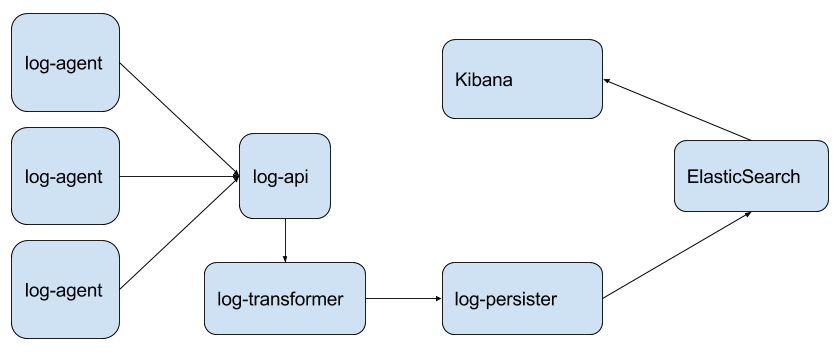
\includegraphics[width=1.0\textwidth]{images/application_arch}
    \caption[Architektura aplikacji]{
        Architektura aplikacji, źródło: opracowanie własne
    }
    \label{chapter:application:architecture:diagram}
\end{figure}

Część praktyczna pracy dyplomowej, przedstawiona na rysunku \ref{chapter:application:architecture:diagram}, 
zaprojektowana została w architekturze rozproszonej - mikro serwisu. Głównym zadaniem takiego rozwiązania
jest rozbicie faktycznej aplikacji na mniejsze programy. Poszczególne części składowe posiadają jedno, 
jasno określone, zadania i jedynie za nie są odpowiedzialne. Niemniej, zasada pojedynczej odpowiedzialności, znana także jako
jeden z wyznaczników dobrej klasy w rozumieniu programowania obiektowego, jest także i tutaj rozumiana w szerszym
kontekście. Pojedynczy serwis współpracuje z innymi. Przykładowa aplikacja mogłaby realizować funkcjonalność 
sklepu internetowego. Jednymi z wielu zamkniętych w środków serwisów, mogłyby by być te odpowiedzialne za zarządzania
klientami lub ogólnie użytkownikami oraz te, których zadaniem byłoby, wsparcie w kierunku zarządzania towarami oferowanymi
przez sklep. Oba, z kolei, wymagałyby wsparcia kolejnego serwisu - bazy danych. Z przedstawionego opisu wynikają jasno pewne
szczególne cechy tego typu architektury:
\begin{itemize}
    \item[\textbf{skalowalność}] - konieczność uruchomienia kolejnych serwisów tego samego typu nie jest trudnym zadaniem. Dzięki temu, 
    że są to aplikacje małe, są one jednocześnie łatwe w zarządzaniu. Ponadto skalowania w kierunku osi OY jest tańsze. Koszt
    dodania średniej mocy maszyny, na której działałaby kolejne instancja serwisu, jest niższy niż dołożenia szybszych podzespołów
    do już istniejącej maszyny, co jest cechą znamienną skalowania wertykalnego,
    \item[\textbf{nauczenie się aplikacji}] - łatwiej jest zrozumieć prostą aplikację, mechanizmy jej działania, aniżeli dogłębnie poznać
    jedną większą. Okazuje się to szczególnie przydatne w dynamicznych zespołach programistów, gdzie rotacja ludzi jest wysoka albo
    częstym zmianą podlegają wymagania,
    \item[\textbf{lepsze izolowanie}] - żaden program nie jest wolny od błędów. Izolowania poszczególnych serwisów jest szczególnie
    przydatne, jeśli dana aplikacja ma problemy z zarządzaniem pamięcią lub przestrzenią dyskową. Inwestygacja mająca 
    na celu ustalenie problemu w dużym programie zajęłaby dużo więcej czasu, nie wspominając już o jego wyeliminowania. 
    W małych aplikacjach ilość wzajemnych korelacji między poszczególnymi jej komponentami jest znacznie niższa od tej
    spotykanych w średnich i dużych programach,
    \item[\textbf{niezależność}] - model aktualizacji lub bardziej ogólnie przekazywania gotowej aplikacji do środowiska produkcyjnego
    staje się również uproszczony. W architekturze mikro-serwisów, każdy serwis może być rozwijany niezależnie od innych i 
    w takiej samej formie, można wypuszczać jego nowe wersje. Jest to także udogodnienie dla klientów, którzy mogą
    pobrać jedynie mały plik binarny lub archiwum. Sam proces aktualizacji jest również narażony na mniejszą ilość
    trudnych do przewidzenia problemu \cite{microservice_architecture}. 
\end{itemize}

Najważniejszą jednak cechą, z którą borykają się systemy informatyczne, jest wyeliminowania \textbf{single-point-of-failure}.
To angielskie pojęcia, w praktyce oznaczana, wadę architektury systemu lub nawet i aplikacji. Najczęściej jednak odnosi się
ona do systemu jako całości. Umieszczenie w jednym miejscu jednej dużej aplikacji lub kilku mniejszych współpracujących 
między sobą, powoduje powstania newralgicznego punktu całego systemu, który jeśli ulegnie awarii, w najlepszy wypadku spowoduje
jedynie opóźnienie w dostarczaniu potrzebnych usług, a w najgorszym całkowicie wyłączy system. Warto w tym miejscu dodać, że
awarie, nie muszą być wcale spowodowane przez sam program. Sytuacje takie jak wyczerpania się pamięci operacyjnej lub 
zajęcia całej mocy obliczeniowej procesora, stanowią ułamek możliwych niefortunnych komplikacji. Należy tutaj brać pod uwagę
także awarię sprzętu, przerwy w dostawie prądu, a także konieczność przeprowadzania prac serwisów lub wymiany istniejących
komponentów komputera na lepsza.  

\subsection{Proces instalacji}
\label{chapter:application:architecture:installation}
    Część praktyczna, jak zostało wcześniej omówione, została zrealizowana w architekturze mikro-serwisów. Warto w tym miejscu dodać,
    że oprócz komponentów omówionych w poniższych rozdziałach, jest to tak naprawdę rozszerzenie istniejącego rozwiązania typu \textbf{MaaS}
    (\ref{chapter:monitoring_architecture:maas}) - monasca. W przypadku tak dużego systemu, składającego się z wielu elementów, 
    konieczne było opracowanie spójnej metody instalacji. Wybór padł na \textbf{Ansible}. 
    
    \subsubsection{Ansible - Simple IT Automation}
    Ansible jest odpowiedzią na pytania - Jak wdrożyć kompleksowy system na więcej niż jednej maszynie. Architektura tego rozwiązania,
    zakłada przygotowanie pakietów instalacyjnych w relacji 1:1 do komponentu, który ma on instalować. Wspomniany pakiet, istnieje pod nazwą roli.
    Jest to najmniejsza cegiełka w całym ekosystemie. Domem, korzystając w dalszej części z metafory, jest tak zwany \textbf{playbook}.
    
    \begin{figure}[H]
        \centering
        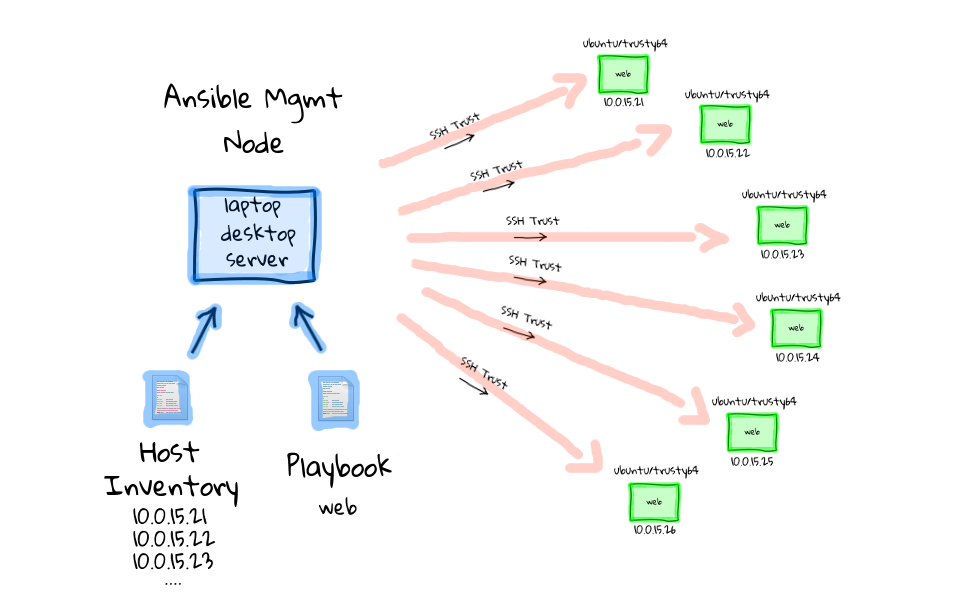
\includegraphics[width=1.0\textwidth]{images/43-ansible-multi-node-deployment-workflow}
        \caption[Wdrożenia z Ansible]{
            Wdrożenia z Ansible, 
            źródło: \url{https://d1cg27r99kkbpq.cloudfront.net/static/extra/43-ansible-multi-node-deployment-workflow.png}
        }
        \label{chapter:application:architecture:installation:ansible_diagram}
    \end{figure}
     
    Pozwala on na budowania scenariusza instalacji według koncepcji przedstawionej na diagramie 
    \ref{chapter:application:architecture:installation:ansible_diagram}. Pojedyncza maszyna, zwana dalej
    maszyną kontrolną, posiada wiedzę o wszystkich hostach wchodzących w skład całego systemu. Na niej
    również zlokalizowane są scenariusze. Ręcznie lub automatyczne zarządzenie infrastrukturą jest
    tutaj aspektem wykraczającym poza ramy pracy dyplomowej, dlatego też nie zostanie omówione. 
    Warto jedynie dodać, że sam proces instalacji na maszynach, możliwy jest do monitorowania na co najmniej
    dwa sposoby:
    
    \begin{itemize}
        \item[Ansible Tower] - rozwiązanie zaprojektowane specjalnie z myślą o monitorowaniu pracy
        procesu wdrożeniowego. Pozwala na przeglądanie listy wszystkich maszyn, obecnego statusu
        zadań (ról),
        \item[Syslog] - wszelka aktywność (tj. operacja), które \textbf{Ansible} wykonuje logowane są
        z użyciem protokołu Syslog na danej maszynie. Dostęp do logów pozwala na prześledzenie operacji oraz
        ewentualnego uzyskania wiedzy na temat przyczyn nieprawidłowego (zakończonego niepowodzeniem) wdrożenia
    \end{itemize}
    
    Najistotniejszą cechą \textbf{Ansible} jest jednak możliwość wskazania, praktycznie nieskończonej,
    ilości maszyn docelowych (fizycznych, wirtualnych lub nawet kontenerów Docker), na których ma zostać ona wprowadzona. 
    Dzięki temu, skalowanie aplikacji na kolejne maszyny, przestaje być operacją problematyczną. Wystarczy dodać 
    informację o jej adresie IP oraz skonfigurować komunikację protokołem SSH.

\section{ELKStack}
\label{chapter:application:elkstack}

\textbf{ELKStack} - akronim opisujący stos technologi składający się z 3 elementów:
\begin{itemize}
    \item[ElasticSearch] - pełnotekstowy silnik wyszukiwania,
    \item[Logstash] - scentralizowane przetwarzania danych,
    \item[Kibana] - interfejs graficzny silnika \textbf{ElasticSearch}
\end{itemize}

\subsection{Logstash}
    Logstash jest wysoce elastycznym narzędziem, nie tylko w kontekście architektury \textbf{ELKStack}.
    Możliwe jest skonfigurowanie go, aby działał jako kolektor danych, jako ich filtr czy też
    transformator. Składa się on z 3 elementów:
    \begin{itemize}
        \item sekcji wejścia,
        \item sekcji przetwarzania,
        \item sekcji wyjścia
    \end{itemize}
    Każda z nich może składać się z więcej niż jednego bloku, opisującego jej zadania.
    Innymi słowy ilość wejść jest nieograniczona tak samo jak możliwości przetworzenia
    odebranych danych oraz ostatecznie wysłania ich do więcej niż jednej lokalizacji.
    Ponadto dla każdej z nich możliwe jest napisania własnego modułu lub wykorzystanie
    jednego z, ciągle rosnącej listy, publicznie dostępnych.
    
    Jest to ponadto rozwiązanie szybkie oraz łatwo skalowalne. Uruchomienie kolejnej
    instancji sprowadza się do przygotowania odpowiedniego pliku konfiguracyjnego
    i dostarczenia go jako argumentu wejściowego do pliku wykonywalnego aplikacji logstash.
    
    \todo[inline]{Opisać korzyści ???}

\subsection{ElasticSearch}
    Pełnotekstowych, indeksowany silnik wyszukiwania. Jednak \textbf{ElasticSearch} jest także
    nierelacyjną bazą danych opartą o koncepcję dokumentów. Możliwość przechowywania oraz wyszukiwania
    informacji pośród zgromadzonych danych, które mogą mieć zarówno ustaloną strukturę, jak i  luźną, jest
    szczególnie istotna dla zarządzania logami. Tym co wyróżnia każdy z nich jest informacja, wiadomość
    zawarta w kolejnych rekordach, a która jest inna dla każdego z nich. 
    
    ElasticSearch oferuje możliwość pełnotekstowej wyszukiwarki na przechowywanych danych, dzięki
    indeksacji. Każda informacja, która wpływa do aplikacji, nie jest po prostu tam zapisywana.
    Specjalnie skonfigurowane indeksy pozwalają na określenie tego, co jest istotne. Ale nie jest
    to konieczne. Jedną z wartych wspomnienia funkcji, jest automatyczna detekcja typów danych, na ich
    podstawie. Wspomniane indeksy są tworzone automatycznie, aby jak najszybciej można było
    wykorzystać możliwości oferowane przez \textbf{ElasticSearch}.
    
    \textbf{Multitenancy}, cecha, wyróżnik chmur obliczeniowych, jest bardzo łatwo do osiągnięcia
    dzięki grupowania i indeksacji w \textbf{ElasticSearch}. Grupa idealnie oddaje koncepcję tenanta.
    Wszystkie dane dla niego zgromadzone mogą zostać odszukane, poprzez wskazania indeksu. Jest on
    tożsamy z grupą, a w dalszej kolejności tenantem.
    
    Jest to także rozwiązania łatwo skalowalne. \textbf{ElasticSearch} posiada ten mechanizm wbudowany.
    Innymi słowy każda nowo uruchomiana instancja poszukuje w sieci, w której działa, innych instancji
    samoistnie budując klaster złożony z lidera oraz replik. 
    Lider odpowiedzialny jest za koordynacją pracy klastra i może również przechowywać dane.
    Repliki stanowią odzwierciedlenie stanu lidera. Jeśli którakolwiek z instancji zostanie wyłączona z klastra,
    potrafi się o samodzielnie przebudować. Dane przesyłane są między replikami. Ostatecznie uzyskuje się
    stan równowagi. Utracenie lidera nie stanowi przeszkody dla poprawnego działania. Pozostałe maszyny 
    negocjują wybór nowego i całość jest ponownie gotowa do świadczenia pełnej funkcjonalności w relatywnie
    krótkim czasie.

    Ostatecznie jest to także \textbf{REST}-owe API. Cała funkcjonalność dostępne jest poprzez
    protokół HTTP. Możliwe jest również administrowaniem klastra przez to samo medium.

\subsection{Kibana}
\label{chapter:application:elkstack:kibana}

    Ostatni z elementów \textbf{ELKStack}. Zadaniem \textbf{Kibana} jest dostarczyć graficznego interfejsu
    użytkownika dla \textbf{ElasticSearch}. Z poziomu aplikacji dostępnej przez przeglądarkę możliwe
    jest przeglądania wszystkich danych zgromadzonych przez \textbf{Logstash} z użyciem tradycyjnych
    metod przeszukiwania:
    \begin{itemize}
        \item filtrowanie,
        \item kwerendy, w tym wypadku pełnotekstowe
    \end{itemize}
    
    Niemniej, to co jest szczególnie użyteczne to wizualizacja danych. Domyślny widok pozwala przeglądać 
    rekordy w formie zbliżonej do tabeli. 
    \begin{figure}[H]
        \centering
        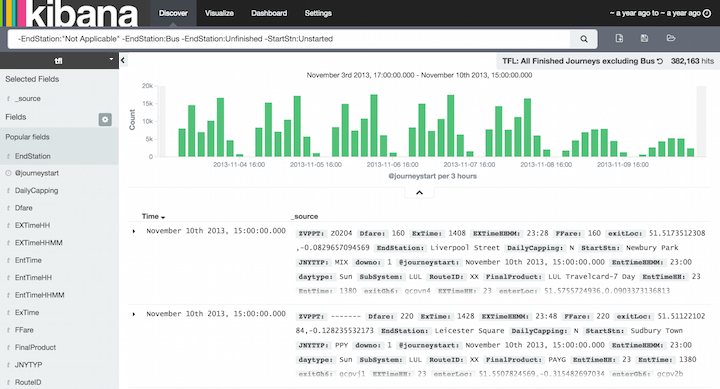
\includegraphics[width=1.0\textwidth]{images/kibana_main_view}
        \caption[Ekran główny w Kibana]{
            Ekran główny w Kibana, źródło: \url{https://www.elastic.co/guide/en/kibana/current/introduction.html}
        }
        \label{chapter:application:elkstack:kibana:main_view}
    \end{figure}
    W tym samym miejscu, można zaobserwować jak Kibana współpracuje z ElasticSearch. Na rysunku \ref{chapter:application:elkstack:kibana:main_view} po lewej stronie widoczny jest pasek szybkiego
    wyszukiwania. Znajdujące się tam pozycje odpowiadają kolejnym właściwościom przeglądanego zbioru danych.
    Korzystając z niego, potencjalny użytkownik, ma możliwość szybkiego filtrowania danych, a ilość filtrów jest
    nieograniczona. Po włączeniu wszystkich szybkiej filtracji, użytkownik w dalszym ciągu, może napisać
    własne zapytania \textbf{QueryDSL} i przesłać je do serwera. Kibana, domyślnie, sortuje dane w kolejności
    rosnącej względem skonfigurowanego pola dla danego indeksu. Rekordy można oglądać w dowolnym wycinku czasu.
    
    Szczególnie interesującą cechą wyników wyszukiwań, które można przeglądać w Kibana, jest to, że bezboleśnie
    łączą się one z dowolną formą wizualizacji. I tak samo, jak użytkownik, mógłby chcieć przejrzeć dane 
    jedynie z konkretnych dwóch godzin, konkretnego dnia, tak samo, możliwe jest uruchomienie podobnego
    filtru dla wykresu kołowego lub słupkowego.
    \begin{figure}[H]
        \centering
        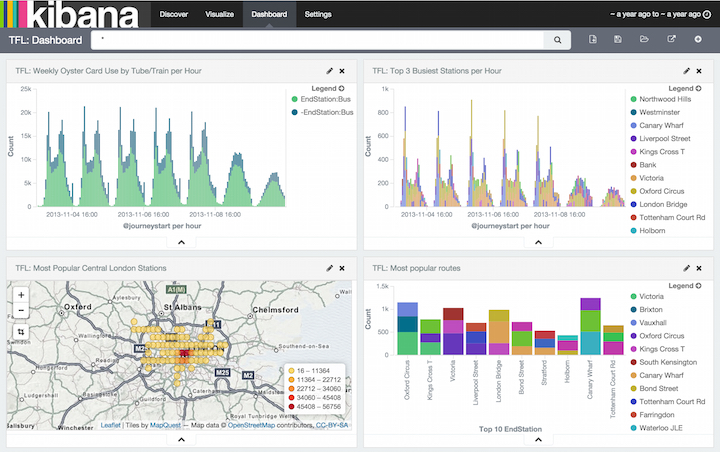
\includegraphics[width=1.0\textwidth]{images/kibana_dashboards}
        \caption[Ekran współdzielony w Kibana]{
            Ekran współdzielony w Kibana, źródło: \url{https://www.elastic.co/guide/en/kibana/current/introduction.html}
        }
        \label{chapter:application:elkstack:kibana:dashboard}
    \end{figure}
    Wykresy, w dalszym ciągu można łączyć w tak zwane \textbf{dashboards}, które stanowią idealne narzędzia do kolaboracji
    w tym samym zespole. Prócz tego, że pozwalają ona na pokazanie jednocześnie więcej niż jednej wizualizacji, z których
    każda odnosi się do samego momentu w czasie, da się je zapisywać i przekazywać innym członkom zespołu. 
\section{monasca-log-agent - zbieranie logów}
\label{chapter:monasca:monasca_log_agent}

    \subsection{Znaczenie komponentu}
    \textbf{monasca-log-agent} jest praktyczną implementacją koncepcji monitorowania aplikacji opartej o agentów.
    Agent zlokalizowany jest więc najbliżej danych, które ma zbierać, a które ma za zadanie przetworzyć i wyniki
    przesłać dalej. Jest to efektywne podejście z uwagi na wolumin danych. Tempo oraz ilość generowanych logów
    może być znacząca, dlatego też pobieranie danych poprzez sieć, znacząco wydłużałoby całkowity czas 
    wszystkich operacji, jakie agent musi wykonać.
    
    \todo[inline]{schemat rozmieszczania agentów, linie schodzą się do monasca-log-api}
    
    Agent został oparty o jeden z elementów stosu technologicznego \textbf{ELKStack} - \textbf{Logstash}.
    Do zadań agenta należy:
    \begin{itemize}
        \item obserwacja wskazanego pliku z logami,
        \item wykrywania i łączenie wpisów składających się z wielu linii,
        \item dodawania informacji o tenancie chmury obliczeniowej,
        \item wskazywania na typ aplikacji, z której logi są zbierane,
        \item wysyłania danych do \textbf{monasca-log-api} \ref{chapter:monasca:monasca_log_api}
    \end{itemize}
    
    Konfiguracja agenta odbywa się w sposób deklaratywny, poprzez plik konfiguracyjny. Poprawne
    skonfigurowanie sprowadza się do:
    \begin{itemize}
        \item wskazania źródła danych,
        \item określenia miejsca docelowego, do którego dane mają zostać wysłane
    \end{itemize}
    W przypadku monitorowania logów, konfiguracja jest bardziej rozbudowane.
    Agent musi zwrócić szczególną uwagę na problem wpisów, które znajdują się w więcej niż jednej linii.
    Najczęściej ten problem objawia się, gdy aplikacja zgłasza błędy, a logach pojawią się rekordy, które
    te problemy opisują. Do opisu błędu (w kontekście logowania) dodawany jest tak zwany \textbf{stacktrace}.
    Zawiera on szczegółowy zrzut wywołań kolejnych funkcji, w różnych modułach, w wyniku których aplikacja
    nie wykonała poprawnie danego zadania. \textbf{Stacktrace}, dla łatwości odczytu przez człowieka,
    jest najczęściej reprezentowany w postaci wpisu zajmującego wiele linii. Z punktu widzenia domyślnej
    konfiguracji \textbf{logstash} kolejne linii to zupełnie odrębne wydarzenia. Dla administratora systemu jest
    to jednak logicznie spójna całość, którą on sam analizował by w takim kontekście. Agent musi więc wiedzieć,
    w jaki sposób połączyć oddzielnie linie w jedno i w takiej formie przesłać je do wyjścia.
    
    \subsection{Problem wielu linii}
    
    \subsection{Konfiguracja agenta}
        \todo[inline]{przykładowa konfiguracja}
        
        \subsubsection{Obserwacja wskazanego pliku z logami}
            Do konfiguracji logstash'a przekazywana jest ścieżka lub wyrażenia regularnego wskazującego
            na, odpowiednio, plik lub listę plików, z których odczytywana mają być rekordy. \textbf{Logstash}
            wykonuje to zadanie podobnie do Linuksowego narzędzia \textbf{tail}. Kolejne zdarzenia w danej 
            instancji agenta, to kolejne linii w obserwowanych plikach, pojawiające się na ich końcu. 
        
        \subsubsection{Wykrywania i łączenie wpisów składających się z wielu linii}
            Problem ten rozwiązany jest z użyciem następującego algorytmu:
            \begin{enumerate}
                \item określenie jaki typ aplikacji jest monitorowany,
                \item utworzenia adekwatnego wyrażenia regularnego opisującego początek lub koniec wydarzenia,
                \item określenie kierunku łączenia kolejnych rekordów
            \end{enumerate}
            \todo[inline]{Ansible i przygotowane szablony dla multiline}
            
        \subsubsection{Dodawania informacji o tenancie chmury obliczeniowej}
            Agent, jak zostało to wcześniej wspomniane, działa na konkretnej maszynie. Jedną z jej własności jest
            informacja o użytkowniku - tenancie - unikatowy numer UUID. W przypadku logowania jako serwisu,
            szczególnie istotna jest wiedza właśnie o użytkowniku chmury, na rzecz którego, dane logi zostały
            zebrane. \textbf{monasca-log-agent} rozwiązuje ten problem z wykorzystaniem biblioteki \textbf{keystone}
            \footnote{Keystone - aplikacja mająca za zadania rozwiązać problem autentykacji oraz autoryzacji w
                chmurach obliczeniowych Openstack}. 
            Agent, tuż przed przesłanie logu do \textbf{monasca-log-api} wykonuje procedurę logowania do chmury
            używając, dostarczonych w konfiguracji, nazwy użytkownika oraz hasła. Jako wynik, jeśli logowanie 
            zakończyło się sukcesem, otrzymuje token oraz numer tenanta. Dołączony jest on do logu.
            
        \subsubsection{Wskazania na aplikację}
            Informacja o logu zostaje wzbogacona o dane, które pozwalają określić typ oraz samą aplikacją.
            
         \subsubsection{Wysyłanie danych do monasca-log-api}
             Wysyłania danych do monasca-log-api jest poprzedzone logowanie do chmury obliczeniowej, jeśli nie
             zostało ono wcześniej wykonane lub jeśli token wygasł. Po udanej autentykacji, kolejne rekordy
             z logu przesyłane są pojedynczo do serwera, gdzie działa \textbf{monasca-log-api}.
\section{monasca-log-api - REST'owe API dla logów}
\label{chapter:monasca:monasca_log_api}

\textbf{monasca-log-api} jest to \textbf{REST}-owe API skonstruowane jako
brama wejściowa do odbierania logów od agentów (instancje \textbf{monasca-log-agent}
\ref{chapter:monasca:monasca_log_agent}).
    
    \subsection{Proces przysyłania danych}
    \begin{figure}[H]
        \centering
        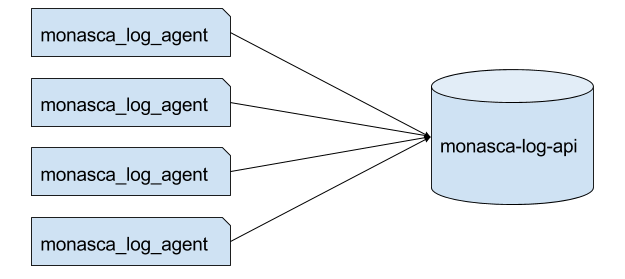
\includegraphics[width=0.80\textwidth]{images/monasca_log_api_data_flow}
        \caption[Relacja monasca-log-agent z monasca-log-api]{
            Relacja monasca-log-agent z monasca-log-api, źródło: opracowanie własne
        }
        \label{chapter:monasca:monasca_log_api:data_flow}
    \end{figure}
    Przesył danych inicjowany jest po stronie agenta. To, co zostanie przesłane
    do \textbf{monasca-log-api}, zależy w dużej mierze od konfiguracji agenta 
    \ref{chapter:monasca:monasca_log_agent:configuration}. Oprócz faktycznego
    logu, agent dodaje najczęściej informacje pozwalające na ustalenie jego pochodzenia (ścieżki, aplikacji) oraz
    datę pobrania rekordu. Po skompletowaniu wszystkich informacji wiadomość podlega
    transformacji do żądania HTTP i zostaje wysłana do serwera.
    
    \subsubsection{Struktura żądania}
    \begin{figure}[h]
        \centering
        
\includegraphics[width=0.80\textwidth]{images/monasca_log_api_request}
        \caption[Żądanie HTTP w monasca-log-api]{
             Żądanie HTTP w monasca-log-api, źródło: opracowanie własne
        }
        \label{chapter:monasca:monasca_log_api:request}
    \end{figure}
    Rysunek \ref{chapter:monasca:monasca_log_api:request} przedstawia przykładowe
    żądanie, jakie agent może wysłać do serwera, w postaci minimalnie wymaganej
    i akceptowanej przez aplikację. Nagłówki żądania:
    \begin{itemize}
        \item \textbf{X-Tenant-Id} - UUID jednoznacznie identyfikujący tenanta w chmurze,
        \item \textbf{X-Application-Type} - wskazuje na typ aplikacji, z której zebrano logi,
        \item \textbf{X-Dimensions} - wszelkie dane opisujące żądanie (nazwa hosta, adres IP hosta itp) 
    \end{itemize}
    stanowią rodzaj uzupełniania dla logu, przesłanego w ciele żądania. Faktyczna ilość nagłówków wygląda 
    jednak inaczej. W wyniku weryfikacji wartości \textbf{X-Tenant-Id}, do listy dołączane są:
    \begin{itemize}
        \item \textbf{X-Identity-Status} - określający status autentykacji,
        \item \textbf{X-Roles} - zestaw uprawnień powiązanych z tenantem.
    \end{itemize}
    
    Również ciało żądania może być dużo większe. Niemniej jest to najczęściej łańcuch tekstowy
    interpretowany jako \textbf{application/json}, który zawierać będzie przynajmniej pole \textbf{message},
    ostatni odczytany wpis w monitorowanego pliku. Na rozmiar żądania natomiast, największy wpływ będzie mieć
    to jak duży był log (na poziomie obserwowanego zasobu). 
    
    Każdy z agentów wysyła kolejne rekordy z monitorowanych plików pojedynczo jako
    ciało żądania HTTP\footnote{Request body lub message body - dane, które klient wysyła do serwera}.
    Zawiera ono surowe dane odczytane przez agenta. \textbf{monasca-log-api} nie zajmuje się normalizacją lub weryfikacją tych danych. Głównym tego powodem jest fakt, że struktura logu na poziomie
    serwera WWW jest rzeczą nieznaną. Wynika to z ilości potencjalnych źródeł, które 
    mogą przesyłać do niego dane. Niemniej walidacja istnieje, ale odnosi się do:
    \begin{itemize}
        \item rozmiaru przesłanych danych (walidacja dwupoziomowa),
        \item nagłówków żądania, które muszę odpowiadać ustalonemu formatowi
    \end{itemize}\cite{monasca_log_api_spec}.
    
    \subsubsection{Proces walidacji}
    \label{chapter:monasca:monasca_log_api:validation}
    
    Serwer nie przetworzy każdego żądania. Jednym z kryterium odrzucenia i
    tym samym walidacji jest rozmiar przesłanych danych. Konieczność wykonania tego kroku, 
    związana jest z elementem odbierającym dane od \textbf{monasca-log-api}, a dokładniej z medium
    którymi informacje są przesyłane. \textbf{Kafka} - kolejka danych - może, w domyślnej konfiguracji,
    przyjąć jednorazowo 1MB (megabajt) danych. \textbf{monasca-log-api} pro-aktywnie eliminuje zbyt duże
    wiadomości, których próba wysłania zakończyłaby się niepowodzeniem. Walidacja odbywa się na dwóch poziomach.
    \begin{itemize}
        \item[Poziom 0] - weryfikowany jest rozmiar samego żądania HTTP. Pod uwagę brany jest nagłówek
        \textbf{Content-Length}, dający informację o ilości (w bajtach) wysłanych przez klienta danych.
        Przekroczenie maksymalnej wartości powoduje wygenerowanie, przez serwer, odpowiedzi 
        \textbf{HTTP 413 :: Request Entity Too Large}. Wspomniany nagłówek jest szczególnie istotny,
        ponieważ pozwala na określenie, czy żądanie można lub nie przetworzyć, bez konieczności
        odczytania właściwych danych. Z tego też powodu, jego brak, również uznawany jest za błąd.
        W odpowiedzi do klienta serwer wygeneruje błąd \textbf{HTTP 411 - Length Required}.
        \item[Poziom 1] - następuje tuż przed wysłaniem wiadomości do \textbf{Kafki}. Po wykonaniu wszystkich
        operacji, związanych z odczytem żądania, dodaniem meta danych do logu, rozmiar wiadomości może się
        znacząco zwiększyć. Możliwa jest sytuacja, w której początkowy rozmiar jest zbliżony do 
        wartości maksymalnej, ale jej nie przekracza. \textbf{monasca-log-api} nie reaguje na poziomie 0. Wiadomość wysyłana do \textbf{Kafki} składa się jednak z większej ilości elementów,
        więc dodawanie ich może spowodować przekroczenie wartości granicznej. W tym wypadku jest to sytuacja
        tożsama z wewnętrznym błędem serwera, w jej wyniku, klient otrzyma odpowiedź
        \textbf{HTTP 500 - Internal Server Error}.
    \end{itemize}
    
    Warto w tym miejscu zaznaczyć, że zmiany w konfiguracji Kafki, odnoszące się do zwiększania
    maksymalnego rozmiaru wiadomości, są również odzwierciedlane w \textbf{monasca-log-api}. 
    
    \subsection{Dostarczanie danych}
    \begin{figure}[H]
        \centering
        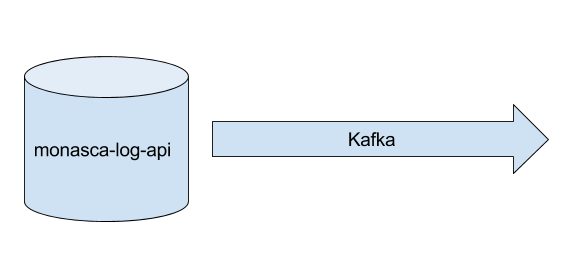
\includegraphics[width=0.80\textwidth]{images/monasca_log_api_to_kafka}
        \caption[monasca-log-api a Kafka]{
            monasca-log-api a Kafka, źródło: opracowanie własne
        }
        \label{chapter:monasca:monasca_log_api:kafka}
    \end{figure}
    Dane z \textbf{monasca-log-api} trafiają do kolejki \textbf{Kafka}.
    Dla każdej z wiadomości obliczana jest specjalna wartość - klucz. Pozwala on na określenia partycji
    wewnątrz Kafki. Dzięki temu dane dystrybuowane są równomiernie. Jest to konieczne z uwagi
    na wolumin danych, które muszą wejść do kolejki. Bez tej operacji mogłoby dojść do przepełnienia się
    bufora wewnątrz Kafki i wiadomości mogłyby zostać utracone. W przypadku logów, o strategicznym
    znaczeniu dla chociażby analizowania przyczyn potencjalnych błędów, jest to sytuacja niedopuszczalna.
    
\section{monasca-log-transformer - proste transformacje}
\label{chapter:monasca:monasca_log_transformer}

\textbf{monasca-log-transformer} jest komponentem znajdującym się bezpośrednio
za \textbf{monasca-log-api}. Jest to ponownie specjalnie skonfigurowana instancje
\textbf{Logstash} \ref{chapter:application:elkstack}. Nasłuchuje on na \textbf{topic}'ach w oczekiwaniu
na wiadomości, które \textbf{monasca-log-api} na nie wysyła. 
\newglossaryentry{kafka_topic}{
    name={Topic},
    description={Topic jest w Kafce tożsamy z grupą. Podczas gdy jedna aplikacja wpisuje dane do wskazanej grupy, inne mogą czytać wiadomości zaadresowane
        do tej grupy. Możliwe jest również czytanie z większej ilości grup}
    }

Po odebraniu wiadomości transformer ma zadanie dokonać, zgodnie z nazwą transformacji, otrzymanego 
logu. Na obecną chwilę jedyną operacją, którą ma za zadanie wykonać jest analiza rekordu pobranego z logu,
aby wykryć jego poziom. Implementacja opiera się na wyrażeniu regularnym, którym objęty jest wycinek
całego logu. W wyniku działania wyrażenia regularnego, do struktury całej wiadomości dodawana jest informacja
o poziomie logu. 

\begin{listing}
    \inputminted[
    fontfamily=monospace,
    fontsize=\scriptsize,
    obeytabs=true,
    samepage=true
    ]{rb}{listingings/transformer.conf}
    \caption[Przykładowa konfiguracja monasca-log-transformer]{
        Przykładowa konfiguracja monasca-log-transformer, źródło: \url{https://raw.githubusercontent.com/FujitsuEnablingSoftwareTechnologyGmbH/ansible-monasca-elkstack/master/templates/transformer.conf.j2}}
    \label{chapter:monasca:monasca_log_transformer:configuration_code}
\end{listing}

Powyższy (\ref{chapter:monasca:monasca_log_transformer:configuration_code}) wycinek kodu przedstawia
sekcję filtracji programu Logstash. Zawarty w niej kod Ruby oraz dopasowanie Grok pozwala na 
pobranie poziomu logu oraz znormalizowania jej do spójnej wartości. 
\section{monasca-log-persister - zapisanie logów do bazy danych}
\label{chapter:monasca:monasca_log_persister}

\textbf{monasca-log-persister} jest ostatnim etapem przed umieszczeniem logów w bazie danych \textbf{ElasticSearch}.
Implementacja została oparta o program \textbf{Logstash}. Prócz zapisu danych do miejsca docelowego, zadaniem
aplikacji jest uzupełnienie logów do postaci, która będzie zrozumiała dla \textbf{ElasticSearch}. 

\begin{listing}
    \inputminted[
    fontfamily=monospace,
    fontsize=\scriptsize,
    obeytabs=true,
    samepage=true
    ]{json}{listingings/persister_input_event.json}
    \label{chapter:monasca:monasca_log_persister:input_message}
    \caption[Przykładowe dane wejściowe dla monasca-log-persister]{
        Przykładowe dane wejściowe dla monasca-log-persister, źródło: opracowanie własne}
\end{listing}

Temu procesowi poddawane są pola takie jak:
\begin{itemize}
    \item[timestamp] - domyślne pole \textbf{@timestamp} generowane jest dla zdarzenia przez \textbf{Logstash}. W przypadku
    logu ważne jest aby ten czas oraz czas, w którym rekord został wygenerowany były tożsame. Dlatego też, program, jeśli
    odnajdzie takową informację w strukturze opisującą log, używa jej jako czasu utworzenia struktury wydarzenia przez instancję
    \textbf{monasca-log-persister}. Dzięki temu, to moment wygenerowania rekordu, jest realnym czasem, według której, w dalszej
    kolejności kolejne pozycje będą sortowane w Kibana.
    \item[creation-time] - znacznik czasowy, wskazujący na odebrania i przetworzenia rekordu przez \textbf{monasca-log-api}.
    \item[dimensions] - \textbf{monasca-log-persister} przenosi wszystkie wartości ustawione w tym polu, do poziomu struktury
    jaką jest zdarzenie.
    \item[application-type] - pole wskazujące na aplikację, która wygenerowała log, podobnie jak \textit{dimensions}, jest przenoszone
    do samego wydarzenia
\end{itemize}

Podobnej operacji podlegają także następujące pola, które oryginalnie zawarte są w logu:
\begin{itemize}
    \item[message] - oryginalna wiadomość, która została pobrana przez \textbf{monasca-log-agent},
    \item[level] - poziom logu przenoszony jest do poziomu wydarzenia jako \textbf{log\_level},
    \item[tenant\_id] - identyfikator użytkownika,
    \item[region] - informacja o regionie, w którym znajdowała się maszyna, a z której pochodzi log,
    \item[path] - ścieżka do pliku, z której pochodzą dane
\end{itemize}
\section{ansible-monasca-kibana}
\label{chapter:application:own_work:ansible_kibana}

    Rola Ansible (\ref{chapter:application:architecture:installation:ansible}) służąca do 
    instalacji klienta stosu \textbf{ELKStack} (\ref{chapter:application:elkstack}), czyli programu Kibana.
    Oprócz wspomnianej instalacji, rola umożliwia również:
    \begin{itemize}
        \item zmianę konfiguracji programu bez konieczności jego ponownej instalacji,
        \item weryfikacją stanu poprzez sprawdzenia zajętości portu TCP,
        \item startowanie oraz zatrzymywanie działania aplikacji
    \end{itemize}
    Dodatkowo rola wspiera mechanizmy izolacji procesów dla platformy Unix. W ramach przygotowania
    do właściwiej instalacji tworzony jest użytkownik oraz grupa. Proces aplikacji uruchamiany będzie później
    pod ich kontrolą, a sam program \textbf{Kibana} posiadał będzie dostęp jedynie do tych zasobów
    systemowych, których właścicielem jest, wspomniany powyżej, użytkownik będący członkiem konkretnej grupy.
    Jest to szczególnie istotne zabezpieczenie, ponieważ zapobiega ona nieautoryzowany dostępowi aplikacji,
    do plików lub innych zasobów systemowych, których nie powinna ona modyfikować.
    
    Całość implementacji przypada autorowi pracy dyplomowej. Kod źródłowy powyższego komponentu jest
    dostępny pod adresem \\ \burl{https://github.com/FujitsuEnablingSoftwareTechnologyGmbH/ansible-monasca-kibana}.

\section{ansible-monasca-elasticsearch}
\label{chapter:application:own_work:ansible_elasticsearch}

    Podobnie jak \textbf{ansible-monasca-kibana} (\ref{chapter:application:own_work:ansible_kibana}), opisywana
    rola służy instalacji jednej z części składowych stosu \textbf{ELKStack} (\ref{chapter:application:elkstack}) - 
    serwera bazodanowego \textbf{ElasticSearch}. Możliwości roli są identyczne do tych opisanych dla roli 
    \textbf{ansible-monasca-kibana}.
    
    Implementacja całej roli jest dziełem autora pracy dyplomowej, a jej kod źródłowy dostępny
    jest pod adresem \burl{https://github.com/FujitsuEnablingSoftwareTechnologyGmbH/ansible-monasca-elasticsearch}.

\section{ansible-monasca-log-transformer}
\label{chapter:application:own_work:ansible_log_transformer}

    W odróżnieniu od \textbf{ansible-monasca-kibana} oraz \textbf{ansible-monasca-elasticsearch}, zadaniem roli
    \textbf{ansible-monasca-log-transformer} jest instalacja na wybranym serwerze, lub serwerach, programu
    \textbf{Logstash} wraz ze specjalną konfiguracją opisaną w rozdziale \ref{chapter:monasca:monasca_log_transformer}.
    
    Dzięki roli możliwe jest:
    \begin{itemize}
        \item zainstalowanie komponentu,
        \item startowanie oraz zatrzymywanie jego działania,
        \item zmiana konfiguracji
    \end{itemize}
    
    Niestety, z uwagi na specyfikę instalowanego programu, którym jest Logstash, nie jest możliwa weryfikacja stanu
    działania aplikacji.
    
    Wstępna implementacja roli jest autorstwa poniższej pracy dyplomowej i może zostać oszacowana na 90\% całego
    kodu źródłowego, który dostępny jest pod adresem
    \burl{https://github.com/FujitsuEnablingSoftwareTechnologyGmbH/ansible-monasca-log-transformer}.

\section{ansible-monasca-log-persister}
\label{chapter:application:own_work:ansible_log_persister}

    Zadaniem omawianej roli jest instalacja programu \textbf{Logstash} wraz z konfiguracją opisaną
    w rozdziale \ref{chapter:monasca:monasca_log_persister}. Funkcjonalność oferowane przez rolę jest
    zbliżone do tej opisanej dla \textbf{ansible-monaca-log-transformer} z jedną szczególną różnicą.
    Możliwe jest zweryfikowanie, czy na wybranym serwerze aplikacja jest działa. Całość weryfikacja oparta jest
    na specyfice komponentu \textbf{monasca-log-persister}. Dane odczytane z kolejki \textbf{Kafka}, po oczyszczeniu
    wysyłane są do serwera \textbf{ElasticSearch}. Aby ta operacja była możliwa, \textbf{Logstash} otwiera konkretny
    port TCP. Zajętość tego portu jest sygnałem, że \textbf{monasca-log-persister} został poprawnie uruchomiony i wysyła
    dane do \textbf{ElasticSearch}.

Całość implementacji przypada autorowi pracy dyplomowej i jest dostępna pod adresem
\burl{https://github.com/FujitsuEnablingSoftwareTechnologyGmbH/ansible-monasca-log-persister}.

\section{ansible-monasca-log-api}
\label{chapter:application:own_work:ansible_monasca_log_api}

    Autor, poniższej pracy dyplomowej, odpowiedzialny był w przypadku omawianej roli głównie za implementację
    logiki, która pozwala by na zainstalowanie \textbf{monasca-log-api} (\ref{chapter:monasca:monasca_log_api}),
    a konkretnie implementacji napisanej w języku Python (\ref{chapter:application:own_work:monasca_log_api:python}).
    
    Rozszerzenie istniejącej roli sprowadziło się do:
    \begin{itemize}
        \item ogólnej poprawy struktury roli poprzez wyodrębnienie odrębnych bloków funkcjonalnych, tworząc
        oddzielne pliki zawierającej ich kod, pozwalających na:
        \begin{itemize}
            \item przygotowanie środowiska do instalacji aplikacji,
            \item właściwego zainstalowania programu na wybranych serwerach lub serwerze,
            \item konfiguracji,
            \item startowania oraz zatrzymywania procesu aplikacji,
            \item weryfikowania stanu
        \end{itemize}
        \item zachowaniu funkcjonalności starej roli, pozwalając w dalszym ciągu na instalację implementacji
        napisanej w języku Java,
        \item dodaniu możliwości instalacji oraz konfiguracji dla implementacji w języku Python
    \end{itemize}
    
    Wkład, twórcy poniższej pracy dyplomowej, ocenić można na około 60\%, a całość kodu źródłowego
    dostępna jest pod adresem \\ \burl{https://github.com/FujitsuEnablingSoftwareTechnologyGmbH/ansible-monasca-log-api}.

\section{Kibana + Keystone}
\label{chapter:application:own_work:kibana_and_keystone}

\textbf{Kibana} domyślnie nie posiada włączonego żadnego mechanizmu autentykacji użytkownika, który
chciałby przeglądać dane, przechowywane w \textbf{ElasticSearch}(\ref{chapter:application:elkstack:elasticsearch}), 
przy jej użyciu. Istnieje prosty mechanizm, który opiera się na standardowym logowaniu przy użyciu
hasła i nazwy użytkownika. Jednakże, z uwagi na późniejsze plany związane z omawianą aplikacją, a które 
omówione zostaną w kolejnym rozdziale, było to rozwiązanie niewystarczające. Fakt ten wynika z natury
integracji, która odbywa się w chmurze obliczeniowej. Konieczne było rozszerzenie Kibany o możliwość
komunikacji z \glslink{keystone}{\textbf{Keystone}}.

Ponieważ dostęp do \textbf{Kibana}, w przypadku tworzonego projektu, dostępny jest z poziomu \glslink{horizon}{\textbf{Horizon}}, inni
członkowie zespołu zajęli się przygotowaniem logiki odpowiedniej dla uruchomienie jej ze wspomnianego miejsca. Autor pracy 
dyplomowej, zaprojektował odpowiedni mechanizm autentykacji zrealizowany według następujących punktów.

    \subsection{Na poziomie serwera}
    W przypadku \textbf{Kibana} należy rozróżnić dwie części składowe - klient oraz serwer. Dodanie autentykacji
    na poziomie warstwy klienta nie byłoby rozwiązaniem poprawnym. Użytkownik końcowy miałby możliwość faktycznego
    uruchomienie strony oraz pobrania danych zanim wykryte by zostało, że nie ma koniecznych do tego uprawnień.
    Wolumin logów, a tym samych danych, które \textbf{Kibana} pobiera z \textbf{ElasticSearch} jest bardzo duży.
    Z tego powodu obciążania komponentów aby zwrócić dane potencjalnie niepotrzebnie zostało
    natychmiastowo wykluczone. Z tego też powodu odpowiednia implementacja znalazła się po stronie serwera.
    
    \subsection{Jako filtr}
    \begin{listing}
        \begin{minted}{js}
app.use('/elasticsearch', require('./lib/keystone'));
        \end{minted}
        \label{chapter:application_own:own_work:kibana_and_keystone:filter_code}
        \caption[Autoryzacja z Keystone w Kibana]{Autoryzacja z Keystone w Kibana, źródło: \url{https://github.com/FujitsuEnablingSoftwareTechnologyGmbH/kibana/blob/master/src/server/app.js}}
    \end{listing}
    Zrealizowana została jako filtr. Jest to specyficzna część aplikacji internetowych, która
    uruchamia się dla wszystkich lub wybranych żądań odbieranych przez serwer.
    
    \begin{listing}
        \begin{minted}{js}
var config = require('../../config');
var express = require('express');

var router = module.exports = express.Router();

if (config.keystone) {
    router.use(require('./auth'));
    router.use(function (err, req, res, next) {
        res.status(err.status || 500);
        res.send({message: err.message});
    });
} else {
    router.use(function (req, res, next) {
        next();
    });
}
        \end{minted}
        \caption[Autoryzacja z Keystone w Kibana - konfiguracja]{Autoryzacja z Keystone w Kibana - konfiguracja, źródło: \url{https://github.com/FujitsuEnablingSoftwareTechnologyGmbH/kibana/blob/master/src/server/lib/keystone/index.js}}
        \label{chapter:application_own:own_work:kibana_and_keystone:filter_configuration}
    \end{listing}
    
    Warto dodać, że pomimo wbudowania filtru do \textbf{Kibana}, nie oznacza to, że musi on być aktywny. Kod
    przedstawiony na listingu \ref{chapter:application_own:own_work:kibana_and_keystone:filter_configuration} oznacza,
    że będzie on włączony jedynie jeśli w pliku konfiguracyjnym dla serwera \textbf{Kibana} znajdzie się odpowiedni
    segment zawierający następujące informacje:
    \begin{itemize}
        \item adres URL serwera \textbf{Keystone},
        \item port dostępu nieuprzywilejowanego,
        \item port dostępu uprzywilejowanego
    \end{itemize}
    
    Filtr posiada jedno wejście i co najmniej dwa, istotne z punktu widzenia omawianego zagadnienia, wyjścia:
    \begin{itemize}
        \item[sukces] - jeśli autoryzacja użytkownika się powiedzie, filtr zwraca logiczną wartość - prawda,
        która jest sygnałem dla dalszego przetwarzania żądania,
        \item[blokada] - sytuacja odwrotna do sukcesu. W tym momencie, żądania zostaje odrzucone
        i pojawia się odpowiedni komunikat informujący użytkownika o zbyt niskich uprawnieniach.
    \end{itemize}
    
    \subsection{Dla komunikacji z ElasticSearch}
    Część serwera \textbf{Kibana} nie zajmuje się jedynie dostarczeniem dostępu do bazy danych
    \textbf{ElasticSearch}. Poza tym, przy jego pomocy, serwowane są media właściwe dla stron internetowych
    (pliki HTML, CSS, JS) lub inne media. Sprawdzania praw użytkowników dla
    każdego z takiego typu żądań okazuje się być wysoce nieefektywne, ponieważ nie ma faktycznego
    przełożenia na aspekt bezpieczeństwa. Z tego tez powodu, jedynie żądania o dane, są wcześniej 
    weryfikowane, aby zezwolić lub zabronić \textbf{Kibana}, i w dalszej kolejności użytkowniki,
    dostępu do nich. Omówione powody, wynikają z natury filtrów, które uruchamiania są dla 
    wszystkich żądań trafiających pod konkretny adres.

Kompletny kod źródłowy aplikacji dostępny jest pod adresem \url{https://github.com/FujitsuEnablingSoftwareTechnologyGmbH/kibana}.

\section{keystone-v3-client}
Omówiona w \ref{chapter:application:own_work:kibana_and_keystone} funkcjonalność, zaimplementowana w \textbf{Kibana}, nie 
byłaby możliwa bez biblioteki do komunikacji z \textbf{Keystone} w aplikacji napisanej w \glslink{node_js}{\textbf{NodeJS}}.
W momencie jej implementacji, żadna z istniejących bibliotek nie wspierała nowej wersji \textbf{Keystone} - \textbf{V3}. 
Było to bodźcem dla napisania własnej, której autor poniższej pracy dyplomowej, jest, na obecną chwilę, jedynym autorem. Zwrot \textit{obecna chwila}
jest tutaj istotny, ponieważ \textbf{biblioteka} została udostępniona publicznie na licencji \textbf{Apache V2}. Skutkiem tego jest to, że
każdy programista z dowolnego miejsca na świecie, może stać się jej współtwórcą. 

Jak zostało wspomniane powyżej, nadrzędnym celem \textbf{keystone-v3-client} jest dostarczenie programistom \textbf{NodeJS} możliwości
komunikacji z nową wersją \textbf{Keystone}. Sam \textbf{Keystone} jest tak naprawdę uruchamiany jako serwer, z którym komunikować się można,
wysyłając żądania HTTP. Lista możliwych żądań jest zbyt długa, aby w pełni ją tutaj przedstawić 
\footnote{Pełna specyfikacja \textbf{Keystone} dostępna jest pod adresem \url{http://developer.openstack.org/api-ref-identity-v3.html}}. Jednak,
dla każdego z możliwych adresów \textbf{keystone-v3-client} udostępnia odpowiednie funkcje, która pozwalają te żądania wykonać.
    \begin{listing}
        \begin{minted}{js}
module.exports.tokens = require('./tokens');
module.exports.service_catalog = require('./service-catalog');
module.exports.endpoints = require('./endpoints');
module.exports.domains = require('./domains');
module.exports.projects = require('./projects');
module.exports.users = require('./users');
module.exports.groups = require('./groups');
module.exports.credentials = require('./credentials');
module.exports.roles = require('./roles');
module.exports.policies = require('./policies');
        \end{minted}
        \caption[Definicja obsługiwanych adresów \textbf{Keystone}]{
            Definicja obsługiwanych adresów \textbf{Keystone} jako moduł NodeJS, źródło: \url{https://github.com/FujitsuEnablingSoftwareTechnologyGmbH/keystone-v3-client/blob/master/lib/keystone/index.js}}
        \label{chapter:application_own:own_work:keystone_v3_client:endpoints}
    \end{listing}

Kompletny kod źródłowy biblioteki dostępny jest pod adresem \url{https://github.com/FujitsuEnablingSoftwareTechnologyGmbH/keystone-v3-client}.
Została ona również opublikowana na \url{https://www.npmjs.com}. 
Opis paczki znaleźć można pod adresem \url{https://www.npmjs.com/package/keystone-v3-client}

\section{monasca-log-api}

\subsection{monasca-log-api - Java}
\label{chapter:application:own_work:monasca_log_api:java}
    Implementacja \textbf{monasca-log-api} pojawiła się jako pierwsza. Była ona suplementem dla \textbf{monasca-api}, również 
    napisanego w Java. Jednakże, podczas gdy drugi z omawianych komponentów służy do pracy z alarmami oraz metrykami, 
    \textbf{monasca-log-api} pozwala na zapisywania logów do bazy danych. Autor pracy dyplomowej, mimo że nie jest 
    oryginalnym autorem tego rozwiązania, miał duży wkład w następujące aspekty implementacji:
    \begin{itemize}
        \item poprawa logiki aplikacji odnośnie dodawania meta danych do odbieranych logów,
        \item naprawa zauważonych błędów,
        \item podniesienie jakości kodu,
        \item lepszą walidacją rozmiaru żądania, tym samym maksymalnego rozmiaru logu
    \end{itemize}
    
    Wkład, autora pracy dyplomowej, dla \textbf{monasca-log-api} w języku Java, można oszacować na 20\%.

\subsection{monasca-log-api - Python}
\label{chapter:application:own_work:monasca_log_api:python}

Odpowiedź na trend w przenoszeniu komponentów, będących częścią chmury obliczeniowej OpenStack, na język Python. Autor, poniższej pracy dyplomowej, jest autorem tej implementacji \textbf{monasca-log-api}. Na obecną chwilę jest ona komplementarna do wersji w języku Java. Całość została oparta o szybki serwer \textbf{Gunicorn} kompatybilny z \glslink{wsgi}{\textbf{WSGI}}. Dzięki
temu aplikacja może zostać łatwo przeniesiona na inną implementacją \textbf{WSGI}, bez większych trudności,
jeśli zajdzie taka potrzeba. Implementacja obejmuje:
\begin{itemize}
    \item przygotowanie całej architektury aplikacji, włącznie z:
    \begin{itemize}
        \item ładowaniem ustawień,
        \item rozłożeniem kodu na logiczne, współpracuje ze sobą, elementy,
        \item klasy odpowiedzialne za obsługę żądań HTTP
    \end{itemize}
    \item utworzeniem logiki odnośnie walidacji nadchodzących wiadomości:
    \begin{itemize}
        \item poprawna struktura nagłówków żądania,
        \item dwu etapowa walidacja rozmiaru wiadomości,
    \end{itemize}
    \item autoryzacja dostępu,
    \item mechanizm weryfikacji stanu (z angielskiego \textbf{healtcheck}),
    \item tworzenia struktury gotowej do przekazania dla \textbf{monasca-log-transformer}
\end{itemize}

Warto w tym miejscu dodać, że \textbf{monasca-log-api}, w języku Python, spotkała się z dużo
większym odzewem ze strony społeczności. Na obecną chwilę, kod aplikacji, ma więcej niż 1 kontrybutora.
Kod, wersji Java oraz Python, znajduje się pod adresem \url{https://github.com/openstack/monasca-log-api/}.
Równolegle do przygotowania implementacji w języku Python, autor pracy dyplomowej, rozszerzył rolę
\textbf{ansible-monasca-log-api} opisaną w rozdziale \ref{chapter:application:own_work:ansible_monasca_log_api}.
Wkład, twórcy pracy magisterskiej, można oszacować na poziomie 95\% dla \textbf{monasca-log-api} w wersji
Python.

\section{ORM dla monasca-api oraz monasca-thresh}
\label{chapter:application:own_work:orm}

Oryginalnie oba z komponentów zostały zaprojektowane z myślą o wsparciu dla relacyjnej bazy danych \textbf{MySQL}. 
Pierwszą z kontrybucji dla \textbf{monasca} było rozszerzenie obsługi baz danych o \textbf{PostgreSQL}. Nie zostało
to jednak osiągnięte poprzez dodania nowego zestawu klas, napisanych z myślą o wsparciu jedynie tej bazy danych. Zamiast
tego, wprowadzono rozwiązanie znane pod nazwą \glslink{frontend}{textbf{ORM}}.
Autor, poniższej pracy dyplomowej, nie jest oryginalnym autorem rozwiązania. Propozycja, która zostało,
przedstawiona społeczności, jest dziełem jednego z programistów projektu. Niemniej, twórca pracy magisterskiej był, w późniejszym czasie,
odpowiedzialny za następujące aspekty tej części całego projektu:

    \subsection{Poprawa jakości i struktury kodu}
    W ramach tego punktu, autor, zajął się między innymi ogólnym podniesienie jakości. Zrealizowane to zostało
    na trzech płaszczyznach:
    \begin{itemize}
        \item[monasca-common]
        Przepisania od nowa modelu mapowania obiektowo-relacyjnego. Warto dodać, że projekt \textbf{monasca-common} stanowi
        wspólną bazę dla wszystkich projektów \textbf{monasca}. Z tego też powodu, model danych zaimplementowany jest
        właśnie w tym projekcie. Nowa wersja warstwy modelu danych cechuje się:
        \begin{itemize}
            \item wspólną bazą dla kluczy głównych, które zdefiniowane są jedynie na poziomie klasy abstrakcyjnej,
            \item jednolitym podejściem do zarządzania obiektami opisujących dane czasowe,
            \item zgodnym z zalecaniami sposobem obliczenia wartości \textit{hashCode} oraz \textit{equals}
            \footnote{\textit{hashCode} oraz \textit{equals} - dwie podstawowe metody implementowane przez każdą klasę w języku Java. Stanowią one
                kluczowy element, między innymi, w pracy z kolekcjami}
        \end{itemize}
        \item[monasca-api, monasca-thresh]
        Dopasowania repozytoriów danych do nowego modelu obiektowego. Największym sukcesem było
        wykorzystanie wstępnie przygotowanych zapytań HQL\footnote{HQL - Hibernate Query Language, jest to
            pseudo obiektowy język zapytań, podobny do SQL}, zamiast tych, które wykorzystywały łączenie
        łańcuchów znakowych. Takie podejście, jest mało eleganckie i trudne w utrzymaniu. Zaletą HQL są
        parametry posiadające własną nazwę. Dodatkowo, tam gdzie było to konieczne i możliwe, autor
        zastosował dynamicznie budowane zapytania, oparte o 
        \href{https://docs.jboss.org/hibernate/orm/5.0/devguide/en-US/html_single/#d5e3489}{Criteria API}.
        Dla potencjalnie dużych zbiorów danych, autor zastosował mechanizm podobny do kursora, aby
        dostarczyć wymaganej funkcjonalności. Ostatecznie był on także autorem poprawek do testów jednostkowych,
        bazujących na tych, które oryginalnie stworzone zostały na potrzeby repozytoriów, komunikujących się
        z \textbf{MySQL}.
    \end{itemize}
    
    \subsection{Dopasowanie rozwiązania do MySQL i PostgreSQL}
    Mimo, że zastosowanym rozwiązaniem był ORM, okazało się, że dopasowanie modelu danych, tak by pasował do 
    schematu bazy danych \textbf{MySQL} oraz \textbf{PostgreSQL}, jest obarczone dużym stopniem trudności. 
    W dużej mierze napotkane przeszkody wynikały z:
    \begin{itemize}
        \item zastosowaniu dla \textbf{MySQL} typów danych SQL właściwych jedynie dla tej bazy danych,
        \item trudną w zamodelowaniu specyficznej struktury oraz zależności między tabelami,
        \item oparciem relacji dla niektórych encji o typ danych UUID
    \end{itemize}
    
    Warto nadmienić, że część ze wspomnianych problemów została zaadresowane również
    w projekcie \href{https://github.com/FujitsuEnablingSoftwareTechnologyGmbH/ansible-monasca-schema}{ansible-monasca-schema}.
    Autor poniższej pracy dyplomowej, był odpowiedzialny za:
    \begin{itemize}
        \item zamianę typu danych \textit{ENUM} na model reprezentacji tego typu wartości, oparty
        o pojedyncza tabelę. Głównymi zaletami tego rozwiązania są:
        \begin{itemize}
            \item zachowanie wymuszania spójności danych,
            \item możliwość modyfikacji stałych poprzez operacji \textbf{INSERT}, \textbf{DELETE} oraz \textbf{UPDATE}. Warto
            dodać, że dla tabeli tego typu zmiany są operacją trywialną. Nie jest to jednak prawda dla wartości ENUM, ponieważ
            wymaga to zmian bezpośredniości na deklaracji DDL danej tabeli
        \end{itemize}
        Warto dodać, że konieczne było zaprojektowanie nowych tabel, aby posiadały jedną tylko kolumnę, będącą jednocześnie
        wartością oraz kluczem głównym. Celowe złamania zasady normalizacji baz danych podyktowane było, koniecznością
        dopasowania modelu danych, aby pasował zarówno do \textbf{MySQL} oraz \textbf{PostgreSQL} oraz, co ważniejsze,
        zminimalizowaniem ilości koniecznych do wprowadzania zmian w \textbf{monasca-api}, na poziomie warstwy dostępu do danych.
        \item zamianą typu danych \textbf{MEDIUMTEXT} na \textbf{LONGTEXT}. Podczas gdy drugi ze wspomnianych typów jest równoważnie
        wspierany dla obu baz danych, \textbf{MEDIUMTEXT} działa prawidłowo jedynie dla \textbf{MySQL}
    \end{itemize}
    
    Ostatecznie, oprócz zmian na poziomie modelu danych oraz schematu bazy danych, autor miał wkład w poprawę oraz udoskonalenie
    kodu warstwy dostępu do danych. Najważniejszymi aspektami tej części było utworzenia odpowiednich klas, implementujących logikę
    biznesową, oryginalnie dostępną jedynie dla \textbf{MySQL}. Podstawowym warunkiem akceptacji ze strony społeczności było
    odzwierciedlania wszystkich założeń zaimplementowanych dla \textbf{MySQL}, tak aby możliwe było wykorzystanie mapowania obiektowo-relacyjnego
    zarówno z bazą danych \textbf{PostgreSQL}, jak i \textbf{MySQL}.
    
    \subsection{Migracja bazy danych w Ansible}
    \label{chapter:application:own_work:orm:ansible_migration}
    Dopełnieniem wprowadzanie \textbf{ORM} dla projektów \textbf{monasca-api} oraz \textbf{monasca-thresh} było spełnienie
    wymagań społeczności odnośnie pakietu migracji danych. Żądania dodania tego typu funkcjonalności było następstwem zmian, jakie
    zostały wprowadzona na poziomie definicji schematu bazy danych dla \textbf{MySQL}. W ramach implementacji, autor poniższej pracy dyplomowej,
    rozszerzył rolę \textbf{ansible-monasca-schema} o skrypt migracyjny, który miał zapewnić:
    \begin{itemize}
        \item zamianę wartości typu \textbf{ENUM} na łańcuchy tekstowe oraz utworzenie dodatkowych tabel
        \item napisanie procedury, której zadaniem było konwersja danych na nowy format przechowywania,
        \item zmiana typów kolumn, które były kompatybilne jedynie z \textbf{MySQL}
    \end{itemize}
    
    \subsection{Oszacowany wkład}
    Z uwagi na duży rozmiar obu wspomnianych projektów oraz liczbę kontrybutorów, trudno jest oszacować procentowy wkład 
    autora pracy dyplomowej. Dodatkowo takie oszacowanie komplikuje fakt, że wprowadzenie warstwy \textbf{ORM} dla 
    \textbf{monasca-api} oraz \textbf{monasca-thresh}, nie są jedynymi kontrybucjami twórcy pracy magisterskiej. Niemniej, 
    łączny wkład autora, wyrażony w postaci metryki \textbf{LOC - Lines of code} przedstawia się następująco:
    \begin{itemize}
        \item dla \textbf{monasca-api} jest to 3890 zmienionych linii kodu,
        \item dla \textbf{monasca-thresh}, ta sama metryka przyjmuje wartość 1589 linii.
    \end{itemize}
    Większość z nich przypada na implementację mapowania obiektowo-relacyjnego.
    Dla roli \textbf{ansible-monasca-schema}, ilość zmienionych linii kodu wynosi 1459. Całość kontrybucji odnosi się do 
    zmian opisanych w rozdziale \ref{chapter:application:own_work:orm:ansible_migration}.

\section{Problem wielu linii w monasca-log-agent}
\label{chapter:application_own:own_work:monasca_log_agent}

    \subsection{Przedstawienie problemu}
    \begin{listing}[h]
        \begin{minted}{yaml}
        {
            name: "multiline",
            type: '"go"',
            configuration: {
                pattern: '"^\[(?!signal)\w+\]"',
                what: '"previous"',
                negate: '"true"'
            }
        }
        \end{minted}
        \caption[Detekcja wielu liniach dla języka GOLang]{
            Detekcja wielu liniach dla języka GOLang, źródło: \url{https://github.com/FujitsuEnablingSoftwareTechnologyGmbH/ansible-monasca-log-agent/blob/master/vars/main.yml}}
        \label{chapter:application_own:own_work:monasca_log_agent:filter_example}
    \end{listing}
    
    W pewnym momencie, stało się jasne, że komponent \textbf{monasca-log-agent} nie wspiera wpisów w logach, znajdujących się 
    w więcej niż jednej linii. Twórca pracy dyplomowej był jednym z dwóch autorów rozwiązania, które implementowały wyżej 
    opisaną funkcjonalność. Z uwagi na fakt, że \textbf{monasca-log-agent} jest specjalnie skonfigurowaną instancją 
    \textbf{Logstash}, całość wdrożenia została umieszczona w roli\textbf{Ansible} - 
    \href{https://github.com/FujitsuEnablingSoftwareTechnologyGmbH/ansible-monasca-log-agent}{ansible-monasca-log-agent}.
    Główną ideą było dodania dodanie zestawu stałych, opisujących konfiguracją segmentu filtracji w \textbf{Logstash}.

    \subsection{Opis rozwiązania}
    Przykładowy kod filtru, widoczny na listingu \ref{chapter:application_own:own_work:monasca_log_agent:filter_example}, 
    wykorzystuje wtyczkę \href{https://www.elastic.co/guide/en/logstash/current/plugins-filters-multiline.html}{multiline} 
    dla aplikacji \textbf{Logstash}. Najistotniejszym elementem, w zaprezentowanym kodzie, jest sekcja 
    \textit{configuration}. Jest to mapowanie w stosunku 1:1, odpowiadające konfiguracji wspomnianego filtra. Poszczególne 
    elementy oznaczają:
    \begin{itemize}
        \item[pattern] - wyrażenie regularne, wykorzystane do dopasowania linii kończącej lub rozpoczynającej wydarzenia, zapisane w wielu liniach,
        \item[what] - wskazuje, czy wartość \textit{pattern}, powinna być wykorzystana do dopasowania pierwszej lub ostatniej linijki odczytanej
        z monitorowanego pliku,
        \item[negate] - ściśle powiązane z dopasowaniem lub jego brakiem. Jeśli, korzystając z wyrażenia regularnego, nie uda się dopasować linii,
        wartość logiczna takiego faktu, powinna zostać odwrócona. Jeśli wyrażenia zwróci fałsz, ustawienie \textit{negate} na \textit{true}, 
        spowoduje, że faktyczną zwróconą wartością będzie logiczna prawda. Innymi słowy, w omawianym przykładzie, kolejne linie są częścią jednego
        logu dopóki, dopóty wyrażenie regularne zwraca logiczny fałsz. 
    \end{itemize}
    
    \begin{listing}[H]
        \begin{minted}{text}
    
       
           
       
           filter {
               
                   if {{ filter.type }} in [tags] {
                       {{ filter.name }} {
                           
                               {{ key }} => {{ val }}
                           
                        }
                    }
                
            }
    
        \end{minted}
        \caption[Wpisanie filtrów do pliku konfiguracyjnego \textbf{Logstash}]{
            Wpisanie filtrów do pliku konfiguracyjnego \textbf{Logstash}, źródło: \url{https://github.com/FujitsuEnablingSoftwareTechnologyGmbH/ansible-monasca-log-agent/blob/master/templates/agent.conf.j2}}
        \label{chapter:application_own:own_work:monasca_log_agent:filter_applying}
    \end{listing}
    
    Wspomniany filtr z listingu \ref{chapter:application_own:own_work:monasca_log_agent:filter_example}, jest w dalszej części 
    umieszczany w pliku konfiguracyjnym \textbf{Logstash} z wykorzystaniem kodu z listingu 
    \ref{chapter:application_own:own_work:monasca_log_agent:filter_applying}. 
    Wartymi omówienia cechami jest tutaj:
    \begin{itemize}
        \item[elastyczność] - sekcja filtracji zostanie umieszczona w wynikowym pliku, tylko jeśli zostaną zdefiniowane jakiekolwiek filtry,
        \item[spójność] - wspomniana w kodzie z listingu \ref{chapter:application_own:own_work:monasca_log_agent:filter_example} 
        sekcja \textit{configuration}, jest w 100 procentach kompatybilna z dostępnymi dla danego filtra opcjami konfiguracyjnymi,
        \item[możliwość rozszerzenia] - kod jest niewrażliwy na ilość potencjalnych filtrów. Jest on zdolny do umieszczania zarówno konfiguracji dla jednego
        filtra, ale potrafi też wpisać 100 innych. 
    \end{itemize}

    \subsection{Oszacowany wkład}
    W kontekście omawianej funkcjonalności, jaką jest rozwiązanie problemu wielu linii w logach, autor, poniższej
    pracy dyplomowej, miał 50\% wkład w całą implementację. 

\section{Rotacja logów}
    W trakcie tworzenie projektu okazało się, że część z wewnętrznie używanych aplikacji, nie obsługuje automatycznej rotacji 
    logów. Jest to operacja, w wyniku której plik logów, po przekroczeniu pewnej wartości granicznej, ulega archiwizacji. 
    Autor, poniższej pracy dyplomowej, był częścią dyskusji, w wyniku której wybrano aplikację \textbf{logrorate}. Całość 
    implementacji, jest już autorstwa twórcy pracy magisterskiej. Została ona utworzone jako rola \textbf{Ansible}. Dzięki 
    temu uzyskano rozwiązania możliwe do zastosowania na dowolnej liczbie hostów.

\section{Ocena kodu tworzonego w społeczności}
    Autor jest obecny w pracach całej społeczności jako \textbf{review}'er wszystkich zmian do dowolnego projektu, 
    niezależnie od tego, czy proponowany kod jest częścią nowej funkcjonalności, czy też jest to naprawa zauważonych błędów i 
    uchybień. Dzięki temu statusowi, ma on możliwość oceny jakości kodu, wskazywania potencjalnych problemów lub zgłaszania 
    niepoprawnej implementacji w stosunku do komponentów zależnych.
    Proces oceny oparty jest o 3, niezależne, od siebie oceny:
    \begin{itemize}
        \item[code review] - odnosi się jedynie do samego kodu. Ocena pozytywna jest sumą elementów takich jak:
        \begin{itemize}
            \item poprawne wykorzystania języka programowania,
            \item efektywne korzystanie ze struktur danych,
            \item poprawne skorelowania nowego kodu ze starym,
        \end{itemize}
        \item[verified] -  ocena poprawności działania. Innymi słowy, funkcjonalność, którą zmiana, wprowadza lub poprawia, powinna działać
        zgodnie z intencją autora oraz, przynajmniej, nie wpływać negatywnie na inne elementy,
        \item[workflow] - jest oceną dosyć specyficzną z uwagi na istnienie wartości \textbf{-1}, którą autor zmiany może przyznać sobie sam.
        Jest to informacja dla osób weryfikujących, że kod nie jest jeszcze gotowy i wymaga dalszej pracy. Z drugiej strony, ocena pozytywna w tej grupie,
        jest najczęściej ostatnią z przyznawanych, która ostatecznie kwalifikuję zmianą jako zaakceptowaną. W wyniku tego, kod, który był
        jedynie propozycją, wchodzi do głównej gałęzi
    \end{itemize}
    Swój wkład w tym aspekcie, autor stara się okazywać w każdym z projektów spod szyldy \textbf{monasca}.

\section{Nominacja do statusu code-reviewer}
    Status \textbf{code-reviewer} jest, niejako, prestiżową rolą, jaką programista, będący obecny na 
    \url{http://review.openstack.org} może mieć. Co ważniejsze, aby uzyskać ten status należy być nominowanym do niego. Sama 
    nominacja pochodzi od innych członków, zrzeszonych wokół konkretnych projektów i jest ona jedynie warunkiem koniecznym. 
    Finalna decyzja leży po stronie osób nadzorujących działania społeczności.
    Warto dodać, że status \textbf{code-reviewer} upoważnia programistę do finalnej akceptacji lub odrzucenia proponowanych 
    zmian. W innym wypadku, możliwe jest jedynie ocena kodu i ewentualne przetestowanie zmiany. Jednak nie możliwe jest 
    ocenienie jej na oceną, które kwalifikowała by zmianę do akceptacji.
\section{Plany rozwoje lub obecnie implementowane}
\label{chapter:application:plans}

Aplikacja do zarządzania logami jest w fazie aktywnego rozwoju. 
Do tej pory udało się osiągnąć relatywnie prostą architekturą, dzięki której
możliwe jest zbieranie logów ze wskazanych maszyn oraz opisania ich
dodatkowymi danymi, pozwalającymi łatwo zidentyfikować skąd i kiedy
zostały pobrane oraz wskazać na ich znaczenie w kontekście monitorowanego systemu.

\subsection{Alarmy a logi}
\label{chapter:application:plans:alarm_on_logs}

Jednym z głównych założeń projektu \textbf{monasca} jest powiadamiania użytkownika o 
sytuacjach krytycznych zaistniałych w systemie. Funkcjonalność realizowana jest na podstawie
metryk, zbieranych z całego systemu. Przekroczenie, założonych przez administratora, wartości
krytycznych, skutkuje wygenerowaniem alarmu. Jednak idea ta, nie może zostać
tak łatwo przełożona na logi. 

    \subsubsection{Idea implementacji}
    \textbf{monasca-agent} jest programem, którego głównym zadaniem jest zbierania metryk z systemu, na którym
    został on zainstalowany. Podejście takie sprawdza się w pełni i właściwie jest jedynym możliwym rozwiązaniem,
    jeśli chodzi o monitoring stanu systemu operacyjnego, maszyny lub aplikacji na nim uruchomionych. Niekoniecznie,
    jest to jednak podejście właściwie dla podobnej analizy w przypadku logów. W rozwiązaniu typu \textbf{LaaS}, 
    jednym z celów jest przesłanie danych do centralnej lokalizacji - archiwizacja. W tym samym punkcie, lub
    przesłane dalej, są one podmiotem analizy. Implementacja będzie, przynajmniej koncepcyjne, zbliżona do \textbf{monasca-agent}.
    
    Możliwe są dwie implementacja:
    \begin{itemize}
        \item[dynamiczna] - potencjalny program miałby być zlokalizowany w za \textbf{monasca-log-transformer} (\ref{chapter:monasca:monasca_log_transformer}).
        Odbierałby on logi ze wspomniane programu, które wysyłane byłyby na ten sam lub inny \glslink{kafka_topic}{\textbf{topic}} i poddawał je prostej analizie. 
        \item[statyczna] - oparta o okresowe pobierania relatywnie małych ilości danych z bazy ElasticSearch (\ref{chapter:application:elkstack:elasticsearch}). 
        Zapytanie oczywiście byłoby zoptymalizowanie na pobranie jedynie tych rekordów, gdzie poziom logu osiągnął zadaną przez operatora wartość.
    \end{itemize}
    
    \subsubsection{Analiza dynamiczna w strumieniu}
    \label{chapter:application:plans:alarm_on_logs:streaming}
    
    \begin{figure}[H]
        \centering
        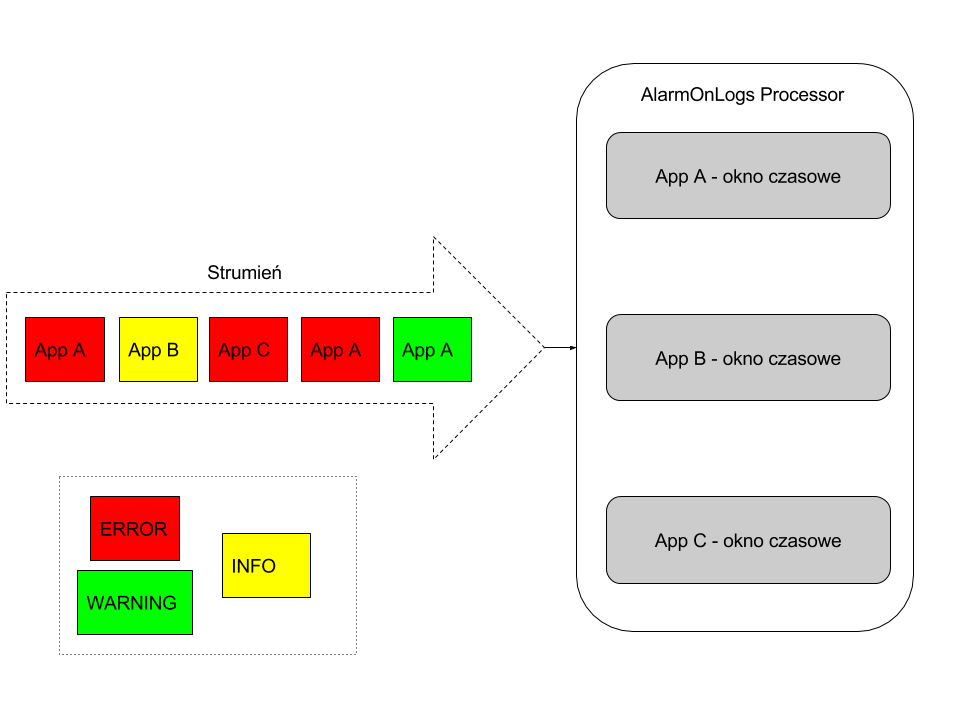
\includegraphics[width=1.0\textwidth]{images/aol_stream}
        \caption[Analiza w strumieniu - schemat]{
            Analiza w strumieniu - schemat, 
            źródło: opracowanie własne
        }
        \label{chapter:application:plans:alarm_on_logs:streaming:diagram}
    \end{figure}
    
    Jest to alternatywa, która idealnie wpisuje się w rzeczywisty charakter danych, jakimi są logami. Ponadto, jest to rozwiązanie, w którym
    wyeliminowana zostaje konieczność iterowanie po zbiorach danych, których wielkość może znacząco spowalniać proces analizy. W programowaniu,
    pętle są najczęściej wskazywane jako najwolniejsze elementy aplikacji, chociaż oczywiście momentami nie da się ich uniknąć. Ponadto, nie ma 
    konieczności także okresowego pobierania danych, co znacząco wydłuża czas odpowiedzi program. Pod uwagę należy jednak wziąć pewne punkty wymagania,
    które musiałyby być spełnione, a które są wyznacznikami przetwarzania w czasie rzeczywistym.
    \begin{itemize}
        \item[ciągły przepływ] - dane, zgodnie z filozofią przetwarzania strumieniowego, muszą przepływać przez aplikację. Wynika z tego, że szybkość
        przetwarzania jest tutaj nadrzędnym celem do osiągnięcia,
        \item[przeciwdziałania strumieniowi] - mimo, że brzmi to jak jeden z antywzorców programowania,
        \footnote{\textbf{Fighting against framework} - próba celowego wykorzystania biblioteki lub wzorca do zadań, do których nie został on zaprojektowany},
        jest to ważna cecha przetwarzania danych w czasie rzeczywistym. Podobnie, jak w rzeczywistym potoku, dane, jak ryby, mogą pływać ławicami, ale mogą
        również napływać pojedynczo, w określonych, i co ważne - nieregularnych, odstępach czasu. Ważne jest więc, aby nie blokować programu, w oczekiwaniu
        na dane. Rozwiązaniem jest zastosowanie mechanizmów takich jak okna przesuwne, których działania powinno się zakończyć po określonym upływie czasu lub
        aktywne nasłuchiwania na pojawiające się dane na wejściu. Szczęśliwie, istnieje odpowiednie biblioteki, które realizuję funkcję aktywnego oczekiwania,
        i wznawiają właściwy wątek programu, jeśli takowa wiadomość nadejdzie. Z drugiej strony, dane mogą napływać dużo szybciej niż aplikacja jest w stanie
        je przetworzyć. W tym wypadku, konieczne może okazać się minimalne buforowanie danych lub przetwarzanie napływających informacji w sposób równoległy.
        \item[powtarzalne rezultaty] - aby silnik alarmujący na podstawie logów generował powtarzalne i, przede wszystkim, 
        spójne rezultaty konieczne jest, aby dane analizować, nie tyle pod kątem poziomu logu, ale także pod względem czasu w jakim został on wygenerowany. 
        Jest to szczególnie istotne, ponieważ system generujący alarm na podstawie tylko jednego punktu wykraczającego poza skalę byłby 
        narażony na zgłaszanie zbyt dużej liczby fałszywych alarmów. Innymi słowy, jeśli system wykryje n-krotne powtórzenie 
        niepoprawnej wartości, powinien wtedy, i tylko wtedy wygenerować alarm. 
        Co prawda, w przypadku logów, omówiona sytuacja, nie zawsze musi być prawdą. Jednostkowe przekroczenie zużycia procesora, nie jest sytuacją anormalną.
        Niemniej, tylko jeden błąd zalogowany przez aplikację o krytycznym znaczeniu może oznaczać błąd. Ale, jeśli program zapisuje w logach jedynie ostrzeżenia,
        dopiero pewna ich liczba, zaobserwowana w, przykładowo, ostatnich 10 minutach działania aplikacji, może zostać uznana, ze problem. Jeśli dane, nie byłyby
        przeglądane pod kątem czasu, w którym powstał wpis, rezultaty analizy byłyby nierzetelne. 10 krotne zaobserwowania wartości \textbf{WARNING} mogłoby tak naprawdę
        pochodzić z próbek wygenerowanych w ciągu ostatnich 30 minutach, a sam fakt, zgłoszenia błędu spowodowany tym, że dotarły one do silnika analizującego
        w oknie czasowym o długości co najwyżej 10 minut \cite{8_requirements_of_real_time_processing}.
        \item[grupowanie] - nie jest to problem, jeśli analizuje się zbiór danych. W danej próbce kontrolnej, dane można łatwo posortować i na jej podstawie 
        wygenerować pewien wynik. Sytuacja komplikuje się dla danych przetwarzanych w potoku. Potencjalny silnik alarmujący otrzymywałby dane pochodzącego z,
        potencjalnie, nieskończonej, liczby różnych programów. Operator, mógłby tak skonfigurować alarmy, aby wykrywać 5 krotne pojawienie się wartości \textbf{ERROR}
        dla aplikacji A, w ciągu 5 minut. Innymi słowy, aplikacja analityczny, musiałaby zapamiętać pojawienia się pierwszego wystąpienia problematycznej wartości.
        Kolejny wymogiem byłoby monitorowanie czasu, jaki upłynął od momentu zauważania wartości po raz pierwszy. Ostatecznie, wygenerowania odpowiedniego,
        alarmu powinna ograniczać się do tych wartości, które wykryto jedynie dla konkretnej aplikacji.
    \end{itemize}
    
    \subsubsection{Analiza tradycyjna na zbiorze}
    \label{chapter:application:plans:alarm_on_logs:bulk}
    
    \begin{figure}[H]
        \centering
        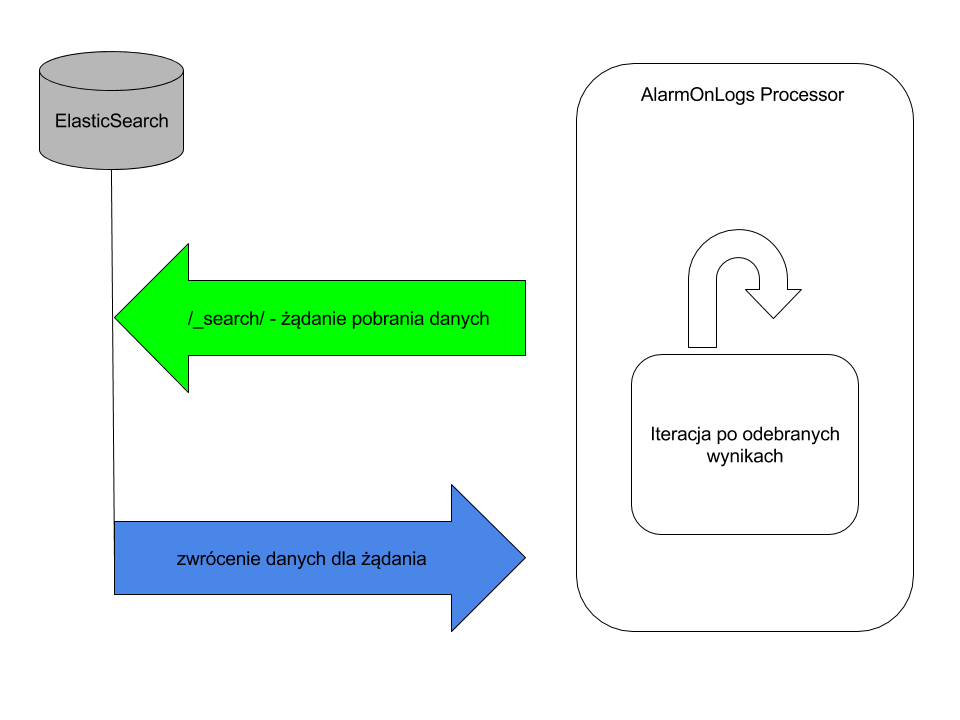
\includegraphics[width=1.0\textwidth]{images/aol_batch}
        \caption[Analiza na zbiorze - schemat]{
            Analiza na zbiorze - schemat, 
            źródło: opracowanie własne
        }
        \label{chapter:application:plans:alarm_on_logs:bulk:diagram}
    \end{figure}
    
    Rozwiązanie alternatywne do omówionego w \ref{chapter:application:plans:alarm_on_logs:streaming}. Rozwiązuje ono wszystkie, przedstawione
    wyżej wymaganie, jakie musiałby spełnić silnik alarmujący, łącznie z grupowaniem. Aplikacja mogłaby pobierać dane, w określonym oknie czasowym,
    ze wskazaniem na poziomu logów oraz aplikacje. Jeśli w odebranych wynikach znalazłyby się odpowiednia
    ilość rekordów, gdzie wartości byłyby przekroczone, byłby to sygnał do wygenerowania alarmu. Niemniej, rozwiązanie tego typu, cechuje się
    narzutem wynikającym z:
    \begin{itemize}
        \item konieczność wygenerowania żądania, otrzymania odpowiedzi i ostatecznie rozpakowania danych do postaci, w której mogłyby zostać
        przetworzone,
        \item program nie może pobierać danych zbyt szybko. Pomijając fakt, że mogłoby to negatywnie wpłynąć na jej wydajność bazy danych, która
        musiałaby przeznaczyć więcej zasobów, aby zrealizować żądanie, wynikałoby to również z konieczności zakończenie przetwarzania już
        otrzymanych danych,
        \item program operowałby na zbiorze, o zmiennej wielkości. Nie byłoby, oczywiście, problematyczne zweryfikowanie małego lub pustego zbioru,
        niemniej otrzymanie dużej ilości rekordów, przełożyłoby się na łączne (czas przesłania, przetworzenia do zrozumiałego formatu, iteracji)
        wydłużenia czasu operacyjnego zaszytego algorytmu. 
    \end{itemize}
    W środowisku, gdzie konieczne jest, szybkie reagowania na ciągle zmieniające się warunki, jakiekolwiek opóźnienia są same w sobie, źródłem
    problemu. Niemniej rozwiązanie to, ma tę szczególną zaletę, że opiera się na istniejącej bazie danych o rozbudowanym API, zdolnym
    zwrócić dane w kompaktowej formie.
    
    Poboczną zaletą obu rozwiązań, jeśli wybranego by oddzielny topic przeznaczony jedynie dla programów analizujących dane, byłoby wykreowania
    swoistej tablicy trasowania (działającej na zasadzie zbliżonej do tej znanej z urządzeń sieciowych), co w dalszej kolejności mogłoby
    służyć do rozdysponowania przekształconych logów do różnych punktów docelowych, gdzie stałyby się one podmiotem całkowicie odrębnych operacji.
    Program miałby za zadania analizować zawartość przesłanych logów. Jeśli poziom, którekolwiek z nich przekroczył by zadaną (skonfigurowaną przez
    administratora lub operatora) wartość, aplikacja tworzyłaby odpowiednią metrykę.
    Obie z implementacji zostały zaproponowane przez autora pracy dyplomowej jako przeciwne do siebie, łącznie z ich zaletami oraz wadami.

    \subsubsection{Metryki nieciągłe}
    W obu przypadkach, niezależnie od przyjętej implementacji, problem jest przedstawienie zebranych danych w postaci metryk - czyli wartości
    numerycznych. W przeciwieństwie do danych dotyczących, chociażby, zużycia przestrzeni dyskowej lub, podlegającemu większej
    fluktuacji, obciążeniu procesora, logi stanowią element zbioru metryk nieciągłych \footnote{Sparse metric - metryki okresowe,
    zwracające wartości w nieregularnych odstępach czasu}. Częścią rozwiązania problemu, byłaby modyfikacja aplikacji \textbf{monasca-thresh},
    odpowiedzialnej za faktyczne generowania alarmów. Na obecną chwilę, jeśli dla danej metryki, brak jest danych, monitor zdefiniowany
    dla danego alarmu powoduje jego wejście w stan \textbf{UNDETERMINED}. W przypadku logów, nie jest to jednak sytuacja oczekiwana. 
    Przykładowo, brak wystąpień błędów dla danej aplikacji, powinien faktycznie oznaczać, że aplikacja lub system pracuje poprawnie i
    potencjalny operator nie ma powodów do niepokoju. Innymi słowy, odpowiadałoby to stanowi \textbf{OK}. Dopiero, co najmniej jedna wartość
    wykraczająca poza ramy danego alarmu, powinna spowodować jego przejście w stan wysoki oraz wygenerowanie powiadomienia lub powiadomień.
\todo[inline]{multitenancy in kibana}
\todo[inline]{keystone authentication as a plugin}

% Na obecną chwilę \textbf{multitenancy} jest jedną z opcji 
% zaplanowanych dla przyszłych wydań projektu. Jednak, komunikacja z \textbf{keystone} jest
% konieczna z innego, niż tylko autoryzacja, powodu. Poboczną korzy